%\documentclass[PhD]{iitmdiss}
%\documentclass[MS]{iitmdiss}
\documentclass[MTech]{iitmdiss}
%\documentclass[BTech]{iitmdiss}
\usepackage{times}
 \usepackage{t1enc}

\usepackage{graphicx} %package to manage images

%\usepackage{graphics}
\usepackage[ruled]{algorithm2e}% http://ctan.org/pkg/algorithm2e
\makeatletter
\renewcommand{\@algocf@capt@plain}{above}% formerly {bottom}
\makeatother
\usepackage{epstopdf}
\usepackage[hypertex]{hyperref} % hyperlinks for references.
\usepackage{amsmath} % easier math formulae, align, subequations \ldots


\begin{document}


%%%%%%%%%%%%%%%%%%%%%%%%%%%%%%%%%%%%%%%%%%%%%%%%%%%%%%%%%%%%%%%%%%%%%%
% Title page

\title{BETWEENNESS CENTRALITY OF A GRAPH}

\author{TEJAS D SHAH}

\date{AUGUST 2017}
\department{COMPUTER SCIENCE AND ENGINEERING}

%\nocite{*}
\maketitle

%%%%%%%%%%%%%%%%%%%%%%%%%%%%%%%%%%%%%%%%%%%%%%%%%%%%%%%%%%%%%%%%%%%%%%
% Certificate
\certificate

\vspace*{0.5in}

\noindent This is to certify that the project titled {\bf BETWEENNESS CENTRALITY OF A GRAPH}, submitted by {\bf TEJAS D SHAH}, to the Indian Institute of Technology, Madras, for
the award of the degree of {\bf Master of Technology }, is a bona fide
record of the project work done by him under our supervision.  The
contents of this report, in full or in parts, have not been submitted
to any other Institute or University for the award of any degree or
diploma.

\vspace*{1.5in}

\begin{singlespacing}
\hspace*{-0.25in}
\parbox{2.5in}{
\noindent Project Guide \\ 
\noindent Professor Rupesh Nasre\\
\noindent Dept. of Physics\\
\noindent IIT-Madras, 600 036 \\
} 
\hspace*{1.0in} 
%\parbox{2.5in}{
%\noindent {\bf Prof.~S.~C.~Rajan} \\
%\noindent Research Guide \\ 
%\noindent Assistant Professor \\
%\noindent Dept.  of  Aerospace Engineering\\
%\noindent IIT-Madras, 600 036 \\
%}  
\end{singlespacing}
\vspace*{0.25in}
\noindent Place: Chennai\\
Date: 31st August 2017 


%%%%%%%%%%%%%%%%%%%%%%%%%%%%%%%%%%%%%%%%%%%%%%%%%%%%%%%%%%%%%%%%%%%%%%
% Acknowledgements
\acknowledgements

Thanks to all those who made this work possible.

%%%%%%%%%%%%%%%%%%%%%%%%%%%%%%%%%%%%%%%%%%%%%%%%%%%%%%%%%%%%%%%%%%%%%%
% Abstract

\abstract

\noindent KEYWORDS: \hspace*{0.5em} \parbox[t]{4.4in}{Betweenneess ; Centrality;
  Graph; BFS; APSP; SSSP.}

\vspace*{24pt}

\noindent 

The betweenness centrality index is essential in the analysis of social networks, but costly to compute. Currently, the fastest known algorithm requires $O(n*m)$ time and $O(n+m)$ space, where $n$ is the number of actors in the network and $m$ is total number of connections amongst them which are unweighted. The existing  Brandes' algorithm does all pairs shortest path and calculates centrality. New algorithms for betweenness of a graph are introduced which tried to improvise the execution time using the same time complexity but failed to do so with respect to existing best available algorithm. However, time complexity has been improved for Trees whereas some execution time improvisation has been achieved if we consider very sparse DAGs.

\pagebreak

%%%%%%%%%%%%%%%%%%%%%%%%%%%%%%%%%%%%%%%%%%%%%%%%%%%%%%%%%%%%%%%%%
% Table of contents etc.



\begin{singlespace}
\tableofcontents
\thispagestyle{empty}

%\listoftables
%\addcontentsline{toc}{chapter}{LIST OF TABLES}
\listoffigures
\addcontentsline{toc}{chapter}{LIST OF FIGURES}
\end{singlespace}


%%%%%%%%%%%%%%%%%%%%%%%%%%%%%%%%%%%%%%%%%%%%%%%%%%%%%%%%%%%%%%%%%%%%%%
% Abbreviations
\abbreviations

\noindent 
\begin{tabbing}
xxxxxxxxxxx \= xxxxxxxxxxxxxxxxxxxxxxxxxxxxxxxxxxxxxxxxxxxxxxxx \kill

\textbf{BC} \> Betweenness Centrality \\
\textbf{APSP} \> All Pairs Shortest Path \\
\textbf{SSSP} \> Single Source Shortest Pat \\
\end{tabbing}

\pagebreak
\pagenumbering{arabic}
%%%%%%%%%%%%%%%%%%%%%%%%%%%%%%%%%%%%%%%%%%%%%%%%%%%%%%%%%%%%%%%%%%%%%%
% Notation

%\chapter*{\centerline{NOTATION}}
%\addcontentsline{toc}{chapter}{NOTATION}

%\begin{singlespace}
%\begin{tabbing}
%xxxxxxxxxxx \= xxxxxxxxxxxxxxxxxxxxxxxxxxxxxxxxxxxxxxxxxxxxxxxx \kill
%\textbf{$r$}  \> Radius, $m$ \\
%\textbf{$\sigma$}  \> Angle of thesis in degrees \\
%\textbf{$\delta$}   \> Flight path in degrees \\
%\end{tabbing}
%\end{singlespace}

%\pagebreak
%\clearpage

% The main text will follow from this point so set the page numbering
% to arabic from here on.



%%%%%%%%%%%%%%%%%%%%%%%%%%%%%%%%%%%%%%%%%%%%%%%%%%
% Introduction.

\chapter{INTRODUCTION}
\label{chap:intro}

In social network analysis, graph-theoretic concepts are used to understand and explain social phenomena. A social network consists of a set of actors, who may be arbitrary entities like persons or organizations, and one or more types of relations between them. An essential tool for the analysis of social networks are centrality indices defined on the vertices of the graph. They are designed to rank the actors according to their position in the network and interpreted as the prominence of actors embedded in a social structure.With the increasing practicality of electronic data collection and, of course, the advent of the Web, there is a likewise increasing demand for the computation of centrality indices on networks with billions of actors.One such centrality is betweeness. 

In graph theory, betweenness centrality is a measure of centrality in a graph based on shortest paths. For every pair of vertices in a connected graph, there exists at least one shortest path between the vertices such that either the number of edges that the path passes through (for unweighted graphs) or the sum of the weights of the edges (for weighted graphs) is minimized. The betweenness centrality for each vertex is the number of these shortest paths that pass through the vertex.
The betweenness centrality of a node $v$ is given by the expression:

\[bc[v] = \sum_{s\neq v \neq t} \sigma_{st}(v) / \sigma_{st}\]

where $\sigma_{st}$ is the total number of shortest paths from node $s$ to node $t$ and $\sigma_{st}(v)$ is the number of those paths that pass through $v$.

Betweenness centrality has also applications in community detection, power grid contingency analysis, and the study of the human brain. However, these analyses come with a high computational cost that prevents the examination of large graphs of interest. Motivated by the fast-growing need to compute centrality indices on large, yet very sparse, networks, new algorithms for betweenness are introduced to reduce the overall execution time. For special graphs such as Trees in specific, the algorithm proposed reduces the execution time by a factor of number of links in the Tree. Whereas, another proposed algorithm reduces execution time for very sparse graphs. 

\section{Brandes' Algorithm}

Given a connected graph $G$, let  $\sigma_{st}$  be the number of shortest paths from a source $s$ $\in$ $V$ to a target $t \in V$ . Let $\sigma_{st} (v)$ be the number of such $s$ $\rightarrow$ $t$ paths passing through a vertex $v \in V $, $v \neq s, t$. Let the pair dependency of $v$ to $s$, $t$ pair be
the fraction $\Delta_{st}(v) =\sigma_{st}(v) / \sigma_{st}$. The betweenness centrality of $v$ is defined by
\begin{equation} \label{eq1}
bc[v]={\sum_{s \neq v \neq t \in V}}  \Delta_{st}(v)   
\end{equation}

Since there are $O$($n^2$) pairs in $V$ , one needs $O$($n^3$) operations to compute $bc[v]$ for all $v \in V$ by using Equation (1.1). Brandes reduced this complexity and proposed an $O(mn)$ algorithm for unweighted networks. The algorithm is based on the accumulation of pair dependencies over target vertices.
After accumulation, the dependency of $v$ to $s \in V$ is 
\vspace{-0.1em}
\begin{equation} \label{eq2}
\Delta_{s}(v) = {\sum_{t \in V}}\Delta_{st}(v)
\end{equation}

Let $P_{s}(u)$ be the set of $u'$s parents on the shortest paths from $s$ to all vertices in $V$. That is,\[  P_{s}(u) = \\{v \in V : (v, u) \in E, d_{s}(u)=_{s}(v)+ 1\\} \]
where $d_{s}(u)$ and $d_{s}(v)$ are the shortest distances from $s$ to $u$ and $v$, respectively.
$P_{s}$ defines the shortest paths graph rooted in $s$. Brandes' observed that the accumulated dependency values can be computed recursively:
\begin{equation} \label{eq3}
\Delta_{s}(v) = \sum_{u:v \in P_{s}(u)} (\Delta_{s}(u)+1)*\sigma_{sv}/\sigma_{su}
\end{equation}
To compute $\Delta_{s}(v)$ for all $v \in V$ except \{$s$\}, Brandes' algorithm uses a two-phase approach: First, a breadth first search (BFS) is initiated from $s$ to compute $\sigma_{sv}$ and $P_{s}(v)$ for each $v$. Then, in a back propagation phase, $\Delta_{s}(v)$ is computed for all $v \in V$ in a bottom-up manner by using Equation (1.3).
In the first phase, the algorithm computes $\sigma[v]$ for $v \in V$ which is the number of shortest paths from the source vertex $s$ to $v$. In addition, the parents of $v$ on these shortest paths are stored in $P[v]$. Before the second phase, the algorithm initializes $\delta[v]$ with 0. 
In the Back propagation phase, the $\delta$  values are calculated and thus are added to the centrality values.

Each phase of Algorithm 1 considers all the edges at most once, taking $O(m + n)$ time. The phases are repeated for each source vertex. The overall complexity is $O(mn)$.

\begin{algorithm}
%\caption{Brandes' Sequential Algorithm}

%\KwResult{Write here the result }
bc[v] $\leftarrow$ 0, $v \in V$\;
\For{$s \in V$}{
$S$ $\leftarrow$ emptystack \;
$P[w] \leftarrow$ empty list, $w \in V$\;
$\sigma[t] \leftarrow$ 0, $t \in V$;  $\sigma[s] \leftarrow$ 1\;
$d[t] \leftarrow$ -1, $t \in V$;  $d[s] \leftarrow$ 0\;
$Q$ $\leftarrow$ emptyqueue \;
enqueue $s \rightarrow Q$ \;
\While{$Q$ not empty}{
dequeue $v \leftarrow Q$\;
Push $v \rightarrow S$\;
\For {neighbour $w$ of $v$}{
\If{$d[w]$ < 0}{
enqueue $w$ $\rightarrow Q$\;
$d[w] \leftarrow d[v]$ + 1\;
}
\If{$d[w] = d[v]$ + 1}{
$\sigma[w] \leftarrow \sigma[w] + \sigma[w]$\;
append $v \rightarrow P[w]$\;
}
}
}

$\delta[v] \leftarrow$ 0, $v \in V$\;


 \While{$S$ not empty}{
 pop $w \leftarrow S$\; 
 \For{$v \in P[w]$}{
 $\delta[v] \leftarrow \delta[v]+ (1+\delta[w])*\sigma[v]/\sigma[w]$\;
 }
  \If{$w \neq s$}{
  $bc[w]= \leftarrow bc[w]+\delta[w]$\;
   }
 }
 }
\end{algorithm}



\chapter{ALGORITHM FOR TREES}
To compute Betweenness Centrality for trees, the Brandes' Algorithm by default will take $O(n^2)$ time where $n$ is total number of vertices of tree.
The proposed algorithm takes $O(n)$ time.
The algorithm is divided into two pass.
\vspace{1em}

\begin{itemize}

  \item Computes number of reachable vertices for each edge of a vertex.
  \item Computes Betweenness Centrality for a vertex using the values computed in first pass.
\end{itemize}

The proposed algorithm is as follows:

The first pass selects any one arbitrary vertex as source and performs Depth First Search(DFS). Every vertex will return to its parent, the number of vertices in its own subtree. The parent vertex will add the returned value from all its children to its own list. So all vertices will have a list of size of their own degree where they will be adding this computed values. The selected source however, will return the total number of vertices in the tree.
So at the at end of first pass, all vertices will have number of vertices in each of its children's subtree.
Total number of vertices = 1 + Number of vertices in each child's subtree + vertices reachable through parent.

In second pass, we will calculate vertices reachable through parent and add it to the list and then calculate the Betweenness Centrality.

Now, since we know total number of vertices reachable from all edges of a vertex, we can calculate Betweenness Centrality using the fact that all the vertices in each subtree has to go through that vertex.



For example if a vertex $v$ has 4 neighbours with number of nodes in each of its subtree as v1,v2,v3,v4 then the list contains v1,v2,v3,v4.
So BC[v]= v1*(v2+v3+v4) + v2*(v3+v4) + v3*v4

Each pass visits each node once and thus the total time complexity of the algorithm is $O(n)$.
%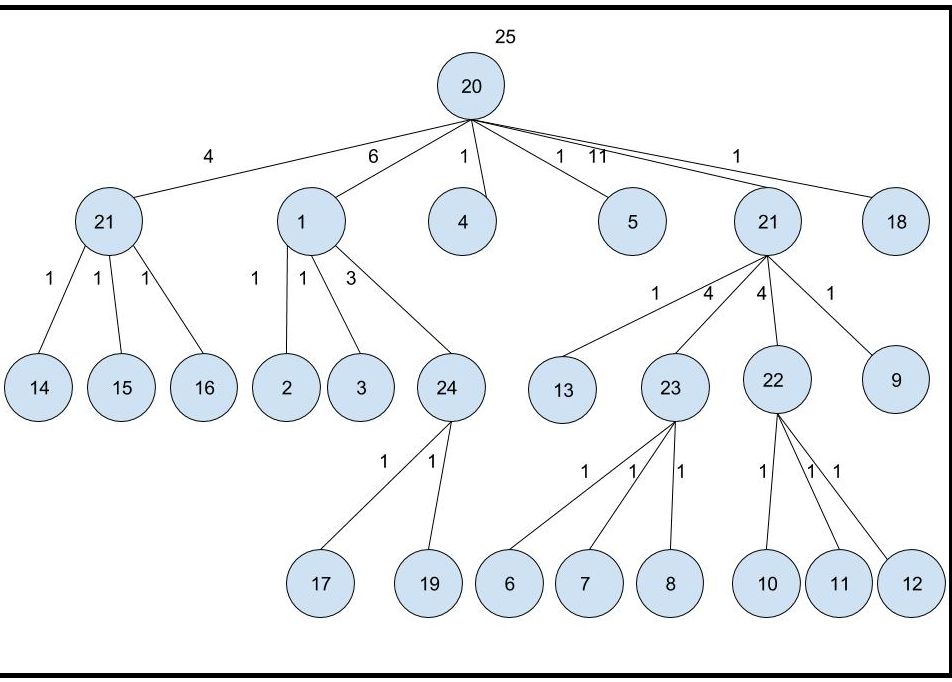
\includegraphics[scale=1.5]{no.jpg}

In the given pseudocode $child$ and $parent$ are the parameters passed to the function dfs. The function returns number of vertices in subtree $child$. 

\begin{algorithm}
%\KwResult{Write here the result }
dfs$($int $child$, int $parent$ $)$ \\
\For{each neighbour vertex $v$ from $child$}{
\If{$v \neq parent$}{
$temp \leftarrow$ dfs($v,child$)\;
$sum \leftarrow sum + temp$\;
Push $sum$ to list[$child$]\;
}
return $sum + 1$\;
}
\caption{First Pass of Tree Algorithm}
\end{algorithm}

\textbf{Proof Of Correctness}
The proposed algorithm is sound because of the fact that for any two vertices, since we are considering only trees there will be exactly one path and by default it will be the shortest. So the centrality value of vertex $v$ is the number of paths going through vertex $v$. The paths going through vertex $v$ will be through one of the edges to other edge. So to calculate the Betweenness Centrality for a vertex $v$ we need to find the total number of reachable vertices from each edge of vertex $v$.



\chapter{ALGORITHM FOR DAGs}

Given a Directed Acyclic Graph $G \equiv (V,E)$ where $V$ is total number of vertices and $E$ is total number of edges. The same algorithm which was proposed for Tree can not be applied here because there may be multiple shortest paths from vertex $s$ to $t$ where $s,t \in V$ in DAG. So we proposed another algorithm for DAG, which reduces the execution time for sparse DAGs.

The first step of the proposed algorithm is to get topological sort and reverse topological sort of the given graph.

The second step will be backward propagation where we will use reverse topological sort computed in first step. At the end of this step, for a vertex $v$, the vertices which are reachable from $v$ and the number of shortest path and its length are stored at vertex $v$. In reverse topological sort, vertex $v$ will push its information to all its parent. Reverse topological sort is used because we are pushing information from a child to a parent so the child's information should be computed first and it should not change as the changed value will propagate to the other vertices. Now, if $(w,u) \in E$ and if the shortest path from $u$ to $v$ is $x$, then from $w$ to $v$ might be $x$ + 1.
But, there may exist other path from $w$ to $v$ which might be shorter than $x$ + 1. In such a case, the information won't be updated at the parent.
If shorter path from $w$ to $v$ is $x$ + 1 with number of paths being $c1$, then the existing number of paths will be incremented by number of paths from $u$ to $v$. If there is still no shorter path or is more than $x$ + 1 from $w$ to $v$ then path length will be $x$ + 1 and number of paths will be that of $u$ to $v$.
After this step, a vertex $v$ will have total number of shortest paths to each reachable vertex from $v$ and their path length.

The third step is to calculate Betweenness Centrality using topological sort computed in first step.For each parent $u$ of vertex $v$, we check whether there is shortest path to all nodes $t$ reachable from $v$ such that distance from $u$ is distance from $v$ + 1. If such a path exists then we will calculate Betweenness Centrality which is given in code.

In pseudocode, $d(v,t)$ is shortest distance calculated in second step from $v$ to $t$ whereas, $c(v,t)$ is count of shortest path from $v$ to $t$.

\vspace{1em}
\begin{algorithm}
%\KwResult{Write here the result }
child $\rightarrow v$, parent $\rightarrow p$ \\
\For{each reachable vertex $t$ from $v$}{
\eIf{$d(v,t) + 1 = d(p,t)$}{
$c(p,t) \leftarrow c(p,t) + 1$\;
}
{
\If{$d(p,t) > d(v,t) + 1$ OR $d(p,t) < 0$}{
$d(p,t) \leftarrow d(v,t) + 1$\;
$c(p,t) \leftarrow c(v,t)$\;
}
}
}
\caption{Second Step of DAG Algorithm}
\end{algorithm}

\vspace{1em}
\begin{algorithm}
%\KwResult{Write here the result }
$bc[v] \leftarrow$ 0, $v \in V$\;
\For{each parent $p$ of vertex $v$}{
\For{each reachable vertex $t$ from $v$}{
\If{$d(v,t) + 1 = d(p,t)$}{
$\Delta_{vt} \leftarrow c(v,t)/c(p,t)$\;
$\sigma_{vt} \leftarrow \sigma_{vt} + \Delta_{vt}*(1 + \sigma_{pt})$\;
$bc[v] \leftarrow bc[v] + \Delta_{vt}*(1 + \sigma_{pt})$\; 
}
}
}
\caption{Third Step of DAG Algorithm}
\end{algorithm}

The issues with this algorithm is that it requires a huge space of since we store count and distance for each reachable vertex $t$ from $v$. Other issue is that the algorithm works well for sparse DAGs but not graphs which dense as many update operations will take up the huge time and deteriorate the execution time.


\chapter{ALGORITHM FOR GRAPHS}

Given a Graph $G \equiv (V,E)$ where $V$ is total number of vertices and $E$ is total number of edges.

Since the proposed algorithm wasn't efficient enough for dense DAGs, hence it was not feasible to apply it for graphs. 
We observed that Brandes' algorithm makes a vertex as a source and performs SSSP for every vertex. But if we select an order such that we can reuse partial graph which will be same for both the vertices. Such an ordering can be if we compute SSSP for vertex $v$ than for any neighbour $u$ of $v$ we can reuse that garph partially, provided that $u$ has yet not been considered for SSSP. And similarly, $u$'s graph can be reused for all its neighbours if they are not considered for SSSP.

For a source $w$, the graph which will be formed while SSSP has edges classified at every vertex as $parent, cousins, children$.
For source $w$, its $parent$ and $cousins$ will remain empty set.
So a vertex $u$ which is not yet considered for SSSP and is neighbour of source $v$ can be ordered such that it becomes next source. So to make SSSP graph of $u$, we will reuse SSSP graph of $v$.

Now to compute SSSP graph of $u$, $u$ becomes the source and its subtree in graph of $v$ remains unchanged. If there is any $cousins$ from subtree to outside of subtree then they will be $children$ in new graph. These newly converted $children$'s $cousins$ will change to $children$.
If there is a edge from a vertex which is not a part of subtree  to a vertex which is part of subtree then they will be cousins.
Hence, we can construct SSSP graph using for $u$ using SSSP graph for $v$.
$\sigma$ values can be easily calculated while making and breaking the links. Then we will apply back propagation phase of Brandes' algorithm to calculate Betweenness Centrality. 

The issues with this algorithm are that it takes up a huge space as we ned to store graphs for each vertex. Also the copying of graphs takes up a lot of time. 












%%%%%%%%%%%%%%%%%%%%%%%%%%%%%%%%%%%%%%%%%%%%%%%%%%%%%%%%%%%%
% Appendices.

%\appendix

%\chapter{A SAMPLE APPENDIX}

%Just put in text as you would into any chapter with sections and
%whatnot.  Thats the end of it.

%%%%%%%%%%%%%%%%%%%%%%%%%%%%%%%%%%%%%%%%%%%%%%%%%%%%%%%%%%%%
% Bibliography.

%\begin{singlespace}
%  \bibliography{refs}
%\end{singlespace}


%%%%%%%%%%%%%%%%%%%%%%%%%%%%%%%%%%%%%%%%%%%%%%%%%%%%%%%%%%%%
% List of papers

%\listofpapers

%\begin{enumerate}  
%\item Authors....  \newblock
% Title...
%  \newblock {\em Journal}, Volume,
%5  Page, (year).
%\end{enumerate}  

\end{document}
